\documentclass[11pt,a4paper]{article}
\usepackage[utf8]{inputenc}
\usepackage[T1]{fontenc}
\usepackage[margin=2.5cm]{geometry}
\usepackage{booktabs}
\usepackage{amsmath}
\usepackage{siunitx}
\usepackage{multirow}
\usepackage{float}
\usepackage[autostyle]{csquotes}
\usepackage[hidelinks]{hyperref}
\usepackage{graphicx}

\sisetup{detect-weight=true}

\title{\bfseries Marocco FL thesis --- week 02/11 update}
\author{}
\date{}

\begin{document}
\maketitle
\vspace{-3.2em}
\begin{center}
\emph{Client-Driven Local Work Assignment in Battery-Constrained Federated Learning}
\end{center}
\vspace{1em}

%======================================================================
\section*{Summary}

\begin{itemize}
  \item The \textbf{v2 campaign} is complete (180 runs, 3 $\beta$ $\times$ 3 seeds):
        SAGE-smart without FedNova, as decided in the call of 30/10, and new
        per-device logs. Against FedAvg ($B=128$) SAGE-smart is more accurate in
        8 pairs out of 9 ($+2.8$ points), uses \textbf{40\,\% less energy in every
        pair} and depletes 8 devices instead of 58. Against the mean of SAGE and
        the ESCS variants it gains 9.7 points with 39\,\% less energy.
  \item \textbf{Where the depletions come from} (Section~\ref{sec:deaths}, as
        requested): even without any training, 8 phones die within 12 hours and
        23 within 26 hours, all of them with medium or heavy use of other apps,
        mostly high-tier phones.
        Of the 9 devices depleted by SAGE-smart (seed 2026), \textbf{7 would die
        anyway}; 84\,\% of their energy went to idle. FedAvg depletes
        \textbf{47 devices more} than the world without FL in the same time,
        including 24 of the 34 low-tier phones, which never die on their own.
  \item \textbf{Equal time and equal accuracy} (Section~\ref{sec:time}): at
        equal elapsed time (11.5~h) SAGE-smart is 8 points above FedAvg but has
        used \textbf{16\,\% more} energy, because it has run 250 rounds against
        109. At equal accuracy it needs \textbf{45\,\% less energy and less than
        half the time} (45\,\%: 582 against 1059~Wh, 5.4 against 11.7~h). The
        energy claim of the thesis should be stated per accuracy reached.
  \item \textbf{Workload experiment} (Section~\ref{sec:workload}): with the load
        of the other apps multiplied by 1.5, 2 and 3, the first version of
        SAGE-smart showed no gain from negotiation and SoC estimate. Diagnosis:
        a busy client accepted and then missed the deadline. In a second version
        (``plus'') the client also refuses when it cannot meet the deadline, and
        the estimate uses the mean reported load. Plus is better at every load
        ($\times3$: 38.9\,\% against 28.6\,\%, 11\,\% less energy, 59 depleted
        devices against 78), and now the negotiation clearly counts. \textbf{For
        now it seems to work, but it is one seed}, and it has a side effect:
        slow phones with large datasets are never selected. A fix is proposed
        and still has to be tested.
  \item The three information protocols (model-first, lightweight, broadcast)
        are written down with their costs (Section~\ref{sec:protocols}).
\end{itemize}

%======================================================================
\section{What changed since the 26/10 report}

\begin{table}[H]
\centering
\small
\caption{Changes since the 26/10 report.}
\label{tab:changes}
\begin{tabular}{p{3.4cm}p{5.6cm}p{6.0cm}}
\toprule
item & now & note \\
\midrule
FedNova & removed from SAGE-smart (call of 30/10) & SAGE-smart aggregates weighted by data, like all the others; all 27 SAGE-smart runs redone \\
v2 campaign & 180 runs, \texttt{results\_..\_v2} & seed 2026 redone for all labels with the new logs; ESCS SP/MD/MP also in the linear and Peukert worlds \\
per-device logs & \texttt{.devsoc}: SoC of every device at every round; \texttt{.devinfo}: tier, workload chain, energy by kind, participations & logging only; present for seed 2026 (all labels) and for all seeds of the labels run in v2 \\
withdrawal cost & a client that receives the model and withdraws pays the download (46~J) and a control message, not the whole exchange (181~J) & 2 withdrawals in the 27 SAGE-smart runs of v2: results unchanged \\
workload multiplier & run parameter \texttt{workload-scale} (label suffix \texttt{\_x3}, \texttt{\_x2}, \texttt{\_x1p5}) & Section~\ref{sec:workload} \\
SAGE-smart ``plus'' & two switches, off by default & Section~\ref{sec:plus}; the v2 runs are unchanged \\
paper & introduction and methodology of the ISLPED draft written & results section still to do \\
\bottomrule
\end{tabular}
\end{table}

FedAvg and FedProx at $\beta=0.1$, seed 2026 were redone because the GPU was
partly occupied at the start of v2: both came back identical to the previous
campaign. Two runs (FedProx $\beta=0.5$ and ESCS-MD $\beta=0.1$, seed 2026)
differ slightly from the previous campaign after round $\sim$130 with the same
code: GPU non-determinism (one sentence in the thesis).

%======================================================================
\section{Results of the v2 campaign}
\label{sec:results}

Same metrics as in the 26/10 report: accuracy = mean over the last 20 rounds;
depleted devices never come back. Only SAGE-smart (no FedNova) and the redone
seed-2026 runs changed; FedAvg, SAGE and ESCS are the same as before.

\begin{table}[H]
\centering
\footnotesize
\caption{Main results, mean over 3 seeds per $\beta$ and mean over the 9 runs.
FedAvg, FedProx and SAGE (paper) in the linear world; the others with the
datasheet battery unless stated.}
\label{tab:main}
\begin{tabular}{lrrrrrrrrrrrr}
\toprule
& \multicolumn{4}{c}{accuracy (\%)} & \multicolumn{4}{c}{energy (Wh)} & \multicolumn{4}{c}{depleted} \\
\cmidrule(lr){2-5}\cmidrule(lr){6-9}\cmidrule(lr){10-13}
$\beta$ & 0.1 & 0.5 & 1.0 & \textbf{all} & 0.1 & 0.5 & 1.0 & \textbf{all} & 0.1 & 0.5 & 1.0 & \textbf{all} \\
\midrule
FedAvg            & 49.9 & 51.8 & 52.9 & 51.5 & 2151 & 2036 & 2004 & 2064 & 58.0 & 58.0 & 58.0 & 58.0 \\
FedProx           & 49.6 & 51.7 & 52.5 & 51.3 & 2151 & 2036 & 2004 & 2064 & 58.0 & 58.0 & 58.0 & 58.0 \\
SAGE (paper)      & 43.6 & 45.7 & 47.0 & 45.5 & 2187 & 2046 & 2094 & 2109 & 35.3 & 34.0 & 27.0 & 32.1 \\
SAGE ablation     & 40.6 & 45.2 & 44.7 & 43.5 & 1963 & 1940 & 1941 & 1948 & 31.0 & 28.7 & 27.0 & 28.9 \\
ESCS-SD           & 42.8 & 45.4 & 45.9 & 44.7 & 1944 & 1982 & 1944 & 1956 & 30.3 & 31.3 & 34.7 & 32.1 \\
ESCS-MD           & 44.3 & 47.8 & 47.7 & 46.6 & 2008 & 2033 & 1983 & 2008 & 33.7 & 36.0 & 32.7 & 34.1 \\
ESCS-SP           & 42.1 & 45.9 & 47.0 & 45.0 & 2209 & 2218 & 2181 & 2203 & 47.0 & 45.0 & 44.3 & 45.4 \\
ESCS-MP           & 40.9 & 45.2 & 44.1 & 43.4 & 2126 & 2094 & 1911 & 2043 & 43.7 & 37.0 & 42.3 & 41.0 \\
\midrule
SAGE-smart (linear)  & 51.1 & 56.4 & 56.0 & 54.5 & 1333 & 1231 & 1228 & 1264 & 10.3 & 6.7 & 5.0 & 7.3 \\
SAGE-smart (Peukert) & 51.4 & 56.2 & 56.2 & \textbf{54.6} & 1288 & 1233 & 1201 & 1241 & 6.3 & 4.3 & 5.0 & \textbf{5.2} \\
SAGE-smart           & 51.1 & 56.3 & 55.6 & 54.4 & 1291 & 1214 & 1202 & \textbf{1236} & 12.0 & 7.0 & 5.7 & 8.2 \\
\bottomrule
\end{tabular}
\end{table}

\begin{table}[H]
\centering
\small
\caption{Paired comparison with FedAvg on the same seed and $\beta$ (9 pairs).
One-sided sign test: 8/9 $p=0.020$, 9/9 $p=0.002$.}
\label{tab:paired}
\begin{tabular}{lrrr}
\toprule
& more accurate than FedAvg & $\Delta$ accuracy (points) & energy saved (min--max) \\
\midrule
FedProx                   & 1/9 & $-0.3 \pm 0.3$ & $0.0\,\%$ \\
SAGE (paper)              & 0/9 & $-6.1 \pm 1.3$ & $-2.3\,\%$ ($-7.7$ to $+2.2$) \\
SAGE ablation             & 0/9 & $-8.0 \pm 2.0$ & $+5.4\,\%$ ($-3.6$ to $+9.7$) \\
ESCS-SD                   & 0/9 & $-6.8 \pm 1.3$ & $+5.0\,\%$ ($-2.0$ to $+10.9$) \\
ESCS-MD                   & 0/9 & $-4.9 \pm 1.7$ & $+2.5\,\%$ ($-4.1$ to $+8.9$) \\
ESCS-SP                   & 0/9 & $-6.5 \pm 1.3$ & $-6.9\,\%$ ($-14.9$ to $-0.6$) \\
ESCS-MP                   & 0/9 & $-8.1 \pm 1.8$ & $+0.9\,\%$ ($-16.1$ to $+8.3$) \\
SAGE-smart (linear)       & \textbf{9/9} & $+3.0 \pm 1.7$ & $+38.7\,\%$ ($+34.9$ to $+42.0$) \\
SAGE-smart (Peukert)      & \textbf{9/9} & $+3.1 \pm 1.6$ & $+39.8\,\%$ ($+36.8$ to $+42.2$) \\
SAGE-smart (datasheet)    & 8/9 & $+2.8 \pm 1.9$ & $\mathbf{+40.1\,\%}$ ($+36.3$ to $+43.3$) \\
\bottomrule
\end{tabular}
\end{table}

\paragraph{What changed with FedNova off.} SAGE-smart (datasheet) goes from
53.9\,\% / 1238~Wh / 8.4 depleted to 54.4\,\% / 1236~Wh / 8.2, and from 7/9 to
8/9 pairs above FedAvg (9/9 with the linear and Peukert batteries). This is
consistent with the cumulative ablation of the 26/10 report, where FedNova cost
1 point. Against the mean of SAGE ablation and the four ESCS variants (datasheet
battery: 44.6\,\%, 2032~Wh, 36 depleted) SAGE-smart gains \textbf{9.7 points
with 39\,\% less energy}.

\paragraph{Energy by kind} (mean of 9 runs). FedAvg: training 945~Wh,
communication 241, idle 878. SAGE-smart: training 435, communication 216, idle
575, state broadcast 10. SAGE and ESCS pay 6--9~Wh of broadcast per run.

%======================================================================
\section{Where the depletions come from}
\label{sec:deaths}

Per-device data: seed 2026, the three $\beta$ (300 devices per method). The
world is the same for all methods with the same seed: 33 high, 33 mid and 34
low-tier phones, and 34 / 33 / 33 phones on the low, medium and heavy workload
chain (other apps: mean load 0.03 / 0.12 / 0.21).

\subsection{Reference: the world without FL}

The same world simulated with no training at all, only idle consumption
($P_{\text{idle}} + w\,(P_{\text{train}}-P_{\text{idle}})$, other apps) and
recharges. Phones die anyway, and always the same ones: heavy users, mostly on
high-tier phones (highest power, 6.15~W at full load).

\begin{table}[H]
\centering
\small
\caption{Devices depleted with no FL at all (seed 2026).}
\label{tab:nofl}
\begin{tabular}{lrrrrrr}
\toprule
hours & 6 & 9 & 12 & 18 & 24 & 30 \\
\midrule
datasheet battery & 0 & 1 & 8 & 19 & 21 & 30 \\
linear battery    & 0 & 1 & 4 & 13 & 18 & 24 \\
\bottomrule
\end{tabular}
\end{table}

\subsection{Depletions per method}

\emph{No FL}: devices that the world without FL loses in the same simulated
time as the run; \emph{due to FL}: the difference (a difference of counts, not
of identities).

\begin{table}[H]
\centering
\footnotesize
\caption{Depleted devices per method, seed 2026, mean over the three $\beta$.}
\label{tab:deaths}
\setlength{\tabcolsep}{4pt}
\begin{tabular}{lrrrrrcc}
\toprule
& duration & depleted & no FL & due to FL & first & by tier & by workload chain \\
& (h) & & & & (h) & high / mid / low & low / medium / heavy \\
\midrule
FedAvg (linear)        & 25.7 & 66.0 & 19.0 & $+47.0$ & 5.9 & 25.0 / 17.0 / 24.0 & 12.7 / 24.0 / 29.3 \\
SAGE (paper, linear)   & 25.3 & 36.0 & 19.0 & $+17.0$ & 7.2 & 16.7 / \phantom{0}9.3 / 10.0 & \phantom{0}0.0 / 13.3 / 22.7 \\
SAGE ablation          & 24.7 & 27.7 & 22.0 & $+5.7$  & 8.2 & 14.0 / \phantom{0}6.7 / \phantom{0}7.0 & \phantom{0}0.0 / \phantom{0}9.3 / 18.3 \\
ESCS-SD                & 22.6 & 33.0 & 21.0 & $+12.0$ & 5.3 & 15.7 / 10.3 / \phantom{0}7.0 & \phantom{0}1.0 / 10.0 / 22.0 \\
ESCS-MD                & 24.0 & 36.3 & 21.3 & $+15.0$ & 6.2 & 17.0 / 10.3 / \phantom{0}9.0 & \phantom{0}0.7 / 13.0 / 22.7 \\
ESCS-SP                & 25.1 & 50.0 & 22.3 & $+27.7$ & 5.1 & 20.7 / 16.0 / 13.3 & \phantom{0}6.0 / 16.7 / 27.3 \\
ESCS-MP                & 25.6 & 43.0 & 22.7 & $+20.3$ & 5.2 & 18.7 / 12.0 / 12.3 & \phantom{0}5.3 / 13.7 / 24.0 \\
SAGE-smart             & 11.5 & 9.0  & 7.0  & $\mathbf{+2.0}$ & 7.6 & \phantom{0}6.7 / \phantom{0}2.3 / \phantom{0}0.0 & \phantom{0}0.0 / \phantom{0}1.3 / \phantom{0}7.7 \\
\midrule
no FL, 25~h (datasheet) & & 23 & & & 7.7 & 13 / 6 / 4 & 0 / 7 / 16 \\
\bottomrule
\end{tabular}
\end{table}

\begin{table}[H]
\centering
\footnotesize
\caption{Who is depleted, final SoC and participation (seed 2026, three
$\beta$). FL share: training + communication + control over the total energy
drawn by the depleted devices. Participations of depleted devices are lower also
because they die before the end.}
\label{tab:who}
\setlength{\tabcolsep}{3.5pt}
\begin{tabular}{lrrrrrrrrr}
\toprule
& FL share & \multicolumn{2}{c}{participations} & \multicolumn{2}{c}{final SoC (\%)} & $<20\,\%$ & participations & never & Gini \\
& depleted & depl. & alive & median & p90 & & per tier h/m/l & selected & \\
\midrule
FedAvg        & 52.7\,\% & 35.2 & 78.8 &  0.0 & 56.9 & 74.7 & 42 / 58 / 50 & 0.0  & \textbf{0.30} \\
SAGE (paper)  & 23.6\,\% & 19.6 & 64.4 & 18.1 & 82.1 & 52.0 & 35 / 55 / 54 & 12.3 & 0.46 \\
SAGE ablation &  8.6\,\% &  6.9 & 55.5 & \textbf{44.0} & 72.5 & 34.0 & 31 / 50 / 45 & 16.7 & 0.43 \\
ESCS-SD       & 33.9\,\% & 30.0 & 60.9 & 27.6 & 81.0 & 45.3 & 49 / 64 / 40 & 2.0  & 0.52 \\
ESCS-MD       & 34.9\,\% & 29.9 & 62.5 & 19.0 & 85.1 & 51.0 & 43 / 64 / 45 & 2.0  & 0.48 \\
ESCS-SP       & 52.8\,\% & 37.3 & 88.8 &  0.2 & 82.4 & 64.3 & 48 / 72 / 69 & 2.0  & 0.43 \\
ESCS-MP       & 51.3\,\% & 34.1 & 71.2 & 18.1 & 89.9 & 51.3 & 43 / 66 / 57 & 2.0  & 0.39 \\
SAGE-smart    & 16.0\,\% & 11.5 & 50.6 & 36.2 & 78.6 & \textbf{21.3} & 43 / 46 / 52 & 3.0 & 0.39 \\
\bottomrule
\end{tabular}
\end{table}

\begin{figure}[H]
\centering
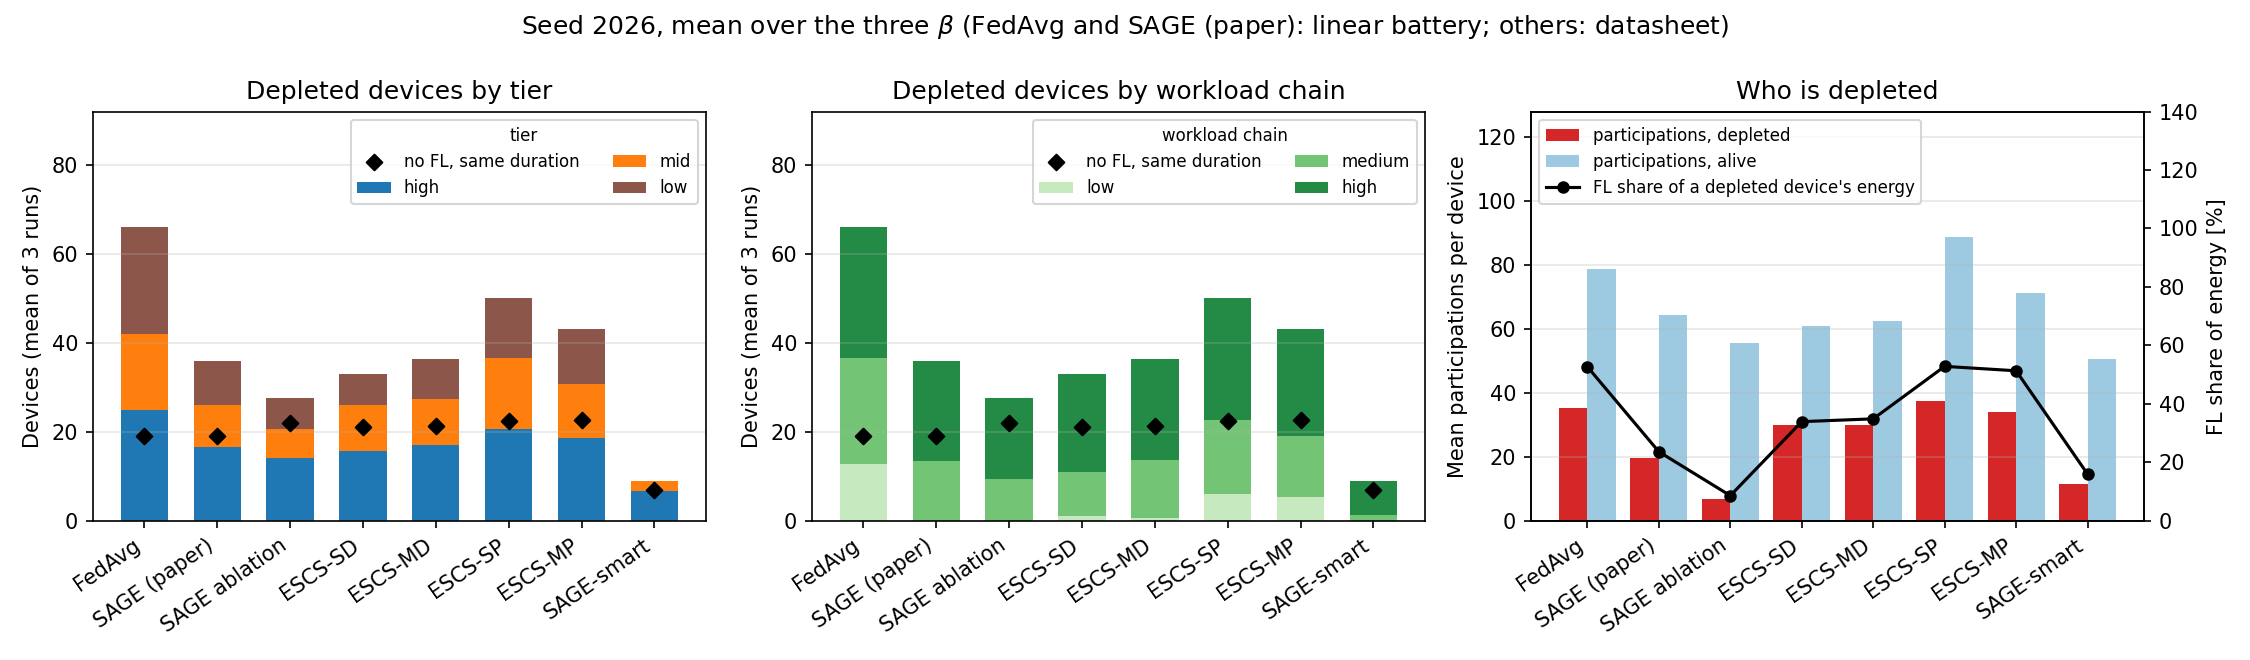
\includegraphics[width=\textwidth]{report14_figs/fig_deaths.png}
\caption{Left and centre: depleted devices by tier and by workload chain; the
diamond is the number that the world without FL loses in the same time. Right:
participations of depleted and surviving devices, and share of a depleted
device's energy that went to FL.}
\label{fig:deaths}
\end{figure}

\begin{figure}[H]
\centering
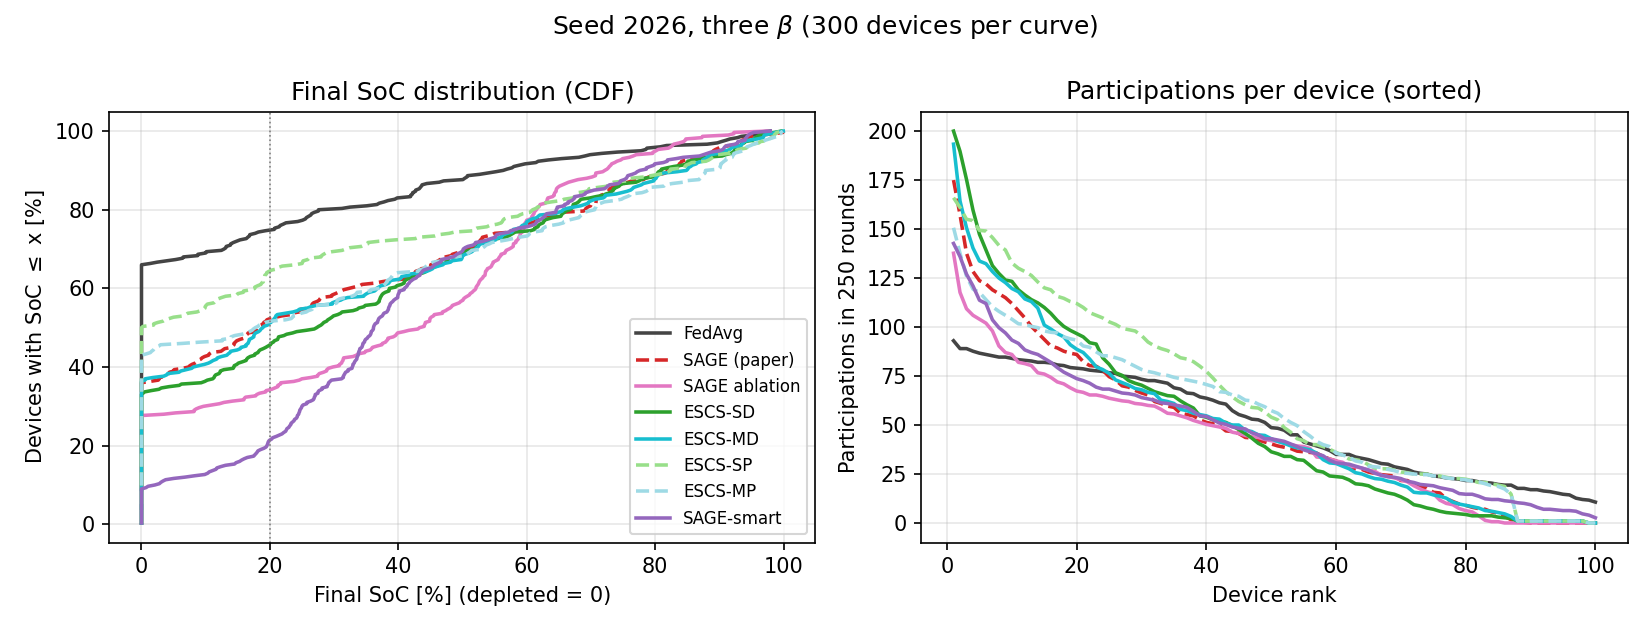
\includegraphics[width=0.92\textwidth]{report14_figs/fig_soc_part.png}
\caption{Final SoC of every device (CDF, depleted = 0) and participations per
device, sorted.}
\label{fig:socpart}
\end{figure}

\paragraph{Reading.}
\begin{itemize}
  \item \textbf{The background kills the heavy users first.} With no FL, the
        first phone dies after 7.7~hours, all deaths are on the medium and heavy
        workload chains, and more than half are high-tier phones. Every method
        loses these phones; the methods differ in how many they add.
  \item \textbf{SAGE-smart adds almost nothing.} 9 depleted devices against 7
        in the world without FL in the same 11.5~h; none of the low tier, none on
        the low workload chain. They were selected 11.5 times on average
        (survivors 50.6) and 84\,\% of their energy went to idle: the score
        stops selecting a device when its SoC falls, and the adaptive epochs keep
        the work small. It also leaves the fewest devices below 20\,\% (21 of
        100, FedAvg 75).
  \item \textbf{FedAvg adds 47 devices}, and kills phones that never die on
        their own: 24 of the 34 low-tier phones and 13 of the 34 phones with
        little background use. With $E=5$ and $B=128$ a low-tier phone trains
        2.2 times longer than a high-tier one for the same work; FedAvg does not
        look at the battery. Half of the energy of its depleted devices went to
        FL.
  \item \textbf{ESCS-SP/MP} add 20--28 devices (they select 46--47 clients per
        round early on); \textbf{SAGE ablation} adds only 6, but it reaches
        only 43.5\,\% accuracy and leaves 17 devices per run never selected.
  \item \textbf{Fairness.} FedAvg (random selection among the alive) has the
        flattest participation (Gini 0.30). SAGE-smart is at 0.39, like ESCS-MP
        and better than SAGE and the other ESCS variants (0.43--0.52). It selects
        low-tier phones slightly more (52 participations against 43 for high-tier
        phones), because high-tier phones lose more charge at idle and have a
        lower SoC. At $\beta=1.0$, 9 devices with a low initial SoC
        (46--59\,\%, all among the 13 lowest) are never selected; at $\beta=0.1$ and 0.5 every device is.
\end{itemize}

%======================================================================
\section{Equal rounds, equal time, equal accuracy}
\label{sec:time}

The 26/10 report noted that the 250 rounds do not last the same time:
11.5~hours for SAGE-smart, 23--26 for the others. With the time column now in
all seed-2026 runs, the three comparisons can be made.

\begin{figure}[H]
\centering
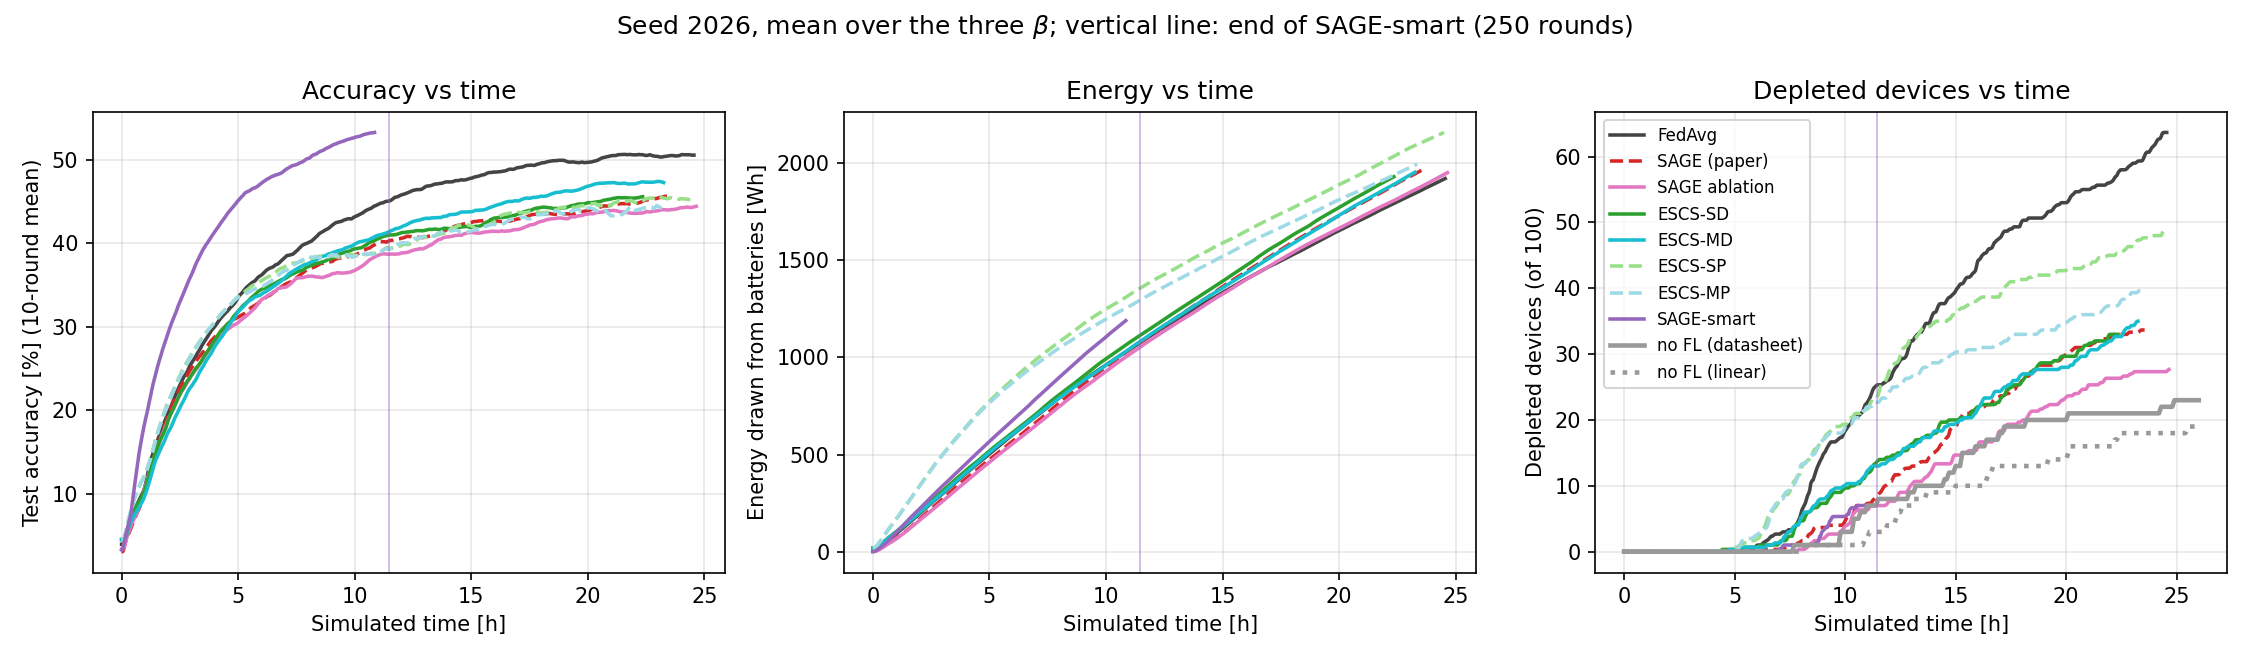
\includegraphics[width=\textwidth]{report14_figs/fig_time.png}
\caption{Accuracy, energy and depleted devices against simulated time (seed
2026, mean over the three $\beta$). Grey: the world without FL.}
\label{fig:time}
\end{figure}

\begin{table}[H]
\centering
\small
\caption{Equal time: every method stopped at the duration of SAGE-smart for
the same $\beta$ (mean 11.5~h), seed 2026, mean over the three $\beta$.
Accuracy: mean of the last 10 rounds before that time. Without FL, 3 (linear)
and 8 (datasheet) devices are depleted at 11.5~h.}
\label{tab:eqtime}
\begin{tabular}{lrrrrr}
\toprule
& rounds done & accuracy (\%) & energy (Wh) & of which idle (Wh) & depleted \\
\midrule
FedAvg         & 109 & 45.5 & \textbf{1072} & 540 & 23.7 \\
SAGE (paper)   & 115 & 40.0 & 1075 & 598 &  9.0 \\
SAGE ablation  & 115 & 38.9 & 1047 & 604 &  \textbf{7.7} \\
ESCS-SD        & 125 & 40.8 & 1107 & 562 & 12.3 \\
ESCS-MD        & 117 & 40.8 & 1079 & 563 & 12.7 \\
ESCS-SP        & 108 & 39.7 & 1352 & 483 & 24.3 \\
ESCS-MP        & 105 & 39.3 & 1289 & 481 & 23.0 \\
SAGE-smart     & 250 & \textbf{53.7} & 1244 & 579 &  9.0 \\
\bottomrule
\end{tabular}
\end{table}

\begin{table}[H]
\centering
\small
\caption{Equal accuracy: energy (9 runs) and simulated time (seed 2026) to
reach a target accuracy (10-round mean). $n$: runs that reach it.}
\label{tab:iso}
\setlength{\tabcolsep}{4pt}
\begin{tabular}{lrrrrrrrrr}
\toprule
& \multicolumn{3}{c}{40\,\%} & \multicolumn{3}{c}{45\,\%} & \multicolumn{3}{c}{50\,\%} \\
\cmidrule(lr){2-4}\cmidrule(lr){5-7}\cmidrule(lr){8-10}
& $n$ & Wh & h & $n$ & Wh & h & $n$ & Wh & h \\
\midrule
FedAvg        & 9/9 &  764 &  8.3 & 9/9 & 1059 & 11.7 & 9/9 & 1607 & 19.2 \\
SAGE (paper)  & 9/9 & 1182 & 11.3 & 5/9 & 1669 & 20.4 & 0/9 & -- & -- \\
SAGE ablation & 8/9 & 1113 & 13.9 & 5/9 & 1578 & 20.6 & 0/9 & -- & -- \\
ESCS-SD       & 9/9 & 1111 & 10.9 & 5/9 & 1604 & 17.2 & 0/9 & -- & -- \\
ESCS-MD       & 9/9 &  971 & 10.4 & 7/9 & 1368 & 15.4 & 0/9 & -- & -- \\
ESCS-SP       & 9/9 & 1291 & 11.3 & 6/9 & 1677 & 16.5 & 0/9 & -- & -- \\
ESCS-MP       & 9/9 & 1333 & 11.4 & 4/9 & 1789 & 17.5 & 0/9 & -- & -- \\
SAGE-smart    & 9/9 & \textbf{436} & \textbf{3.9} & 9/9 & \textbf{582} & \textbf{5.4} & 8/9 & \textbf{764} & \textbf{6.0}$^{*}$ \\
\bottomrule
\multicolumn{10}{l}{\footnotesize $^{*}$ 2 runs of 3 ($\beta=0.1$ does not reach 50\,\% with seed 2026).}
\end{tabular}
\end{table}

\paragraph{Reading.}
\begin{itemize}
  \item \textbf{Equal rounds} (Section~\ref{sec:results}): $-40\,\%$ energy,
        $+2.8$ points.
  \item \textbf{Equal time}: SAGE-smart has done 250 rounds when FedAvg has done
        109, so it is \textbf{8.2 points more accurate} but has drawn
        \textbf{16\,\% more energy} (1244 against 1072~Wh). Per round it uses
        less, but it runs more than twice as many rounds. Idle is about the same
        (480--600~Wh for everybody): it depends on the hours, not on the method.
        The batteries still favour SAGE-smart: 9 depleted against 24 (without
        FL: 8 with the datasheet battery, 3 with the linear one of FedAvg).
  \item \textbf{Equal accuracy}: SAGE-smart reaches 40, 45 and 50\,\% with
        43, 45 and 52\,\% less energy than FedAvg, in less than half the time.
        SAGE and ESCS need more energy than FedAvg for every target and do not
        reach 50\,\%.
  \item \textbf{Consequence for the thesis and the paper}: ``40\,\% less energy
        at 250 rounds'' is true but depends on stopping both at the same round.
        The robust statement is the energy (and time) to reach a given accuracy;
        the battery result (fewer depletions, almost all from the background)
        holds in all three readings.
\end{itemize}

%======================================================================
\section{Information protocols}
\label{sec:protocols}

How the server learns the state of the clients (asked in the call of 30/10).
$N_a=100$ alive clients, $k=20$ selected, $\rho=0.1$ of clients do not answer
a request; a model exchange costs 181~J (ResNet-18, 44.9~MB each way over 4G), a
download alone 46~J, an isolated control session 2.1~J.

\begin{table}[H]
\centering
\small
\caption{Information cost of the three protocols per round (control messages
only; the model exchange of the selected clients is the same for all).}
\label{tab:protocols}
\begin{tabular}{lccc}
\toprule
& P1 model-first & P2 lightweight (SAGE-smart) & P3 broadcast \\
\midrule
who decides $(E,B)$       & client          & client              & server \\
state used                & at training     & at training         & at the broadcast \\
messages before the model & 0               & $k$ + refusals      & $N_a$ \\
energy per refusal        & 46~J (download wasted) & 2.1~J        & -- \\
fixed energy per round    & 0               & $\approx 0$         & $\approx$150~J \\
added latency             & 1 download per refusal & 0.33~s per wave & 1.33~s \\
\bottomrule
\end{tabular}
\end{table}

\begin{itemize}
  \item P2 costs about 20 times less than P1 for each refusal. P1 costs less
        than P3 as long as fewer than $150/46\approx3$ clients refuse per round;
        P2 costs less than P3 unless about 70 clients refuse in the same round.
  \item \textbf{Measured at the nominal load} (v2, 27 SAGE-smart runs): 128\,382
        proposals, 724 refusals (0.56\,\%, 0.1 per round), 2 withdrawals. The
        refusals cost 0.4~Wh in total with P2 (9.3~Wh with P1); the broadcast,
        which is on for SAGE, ESCS and SAGE-smart, costs 10~Wh per run. At this
        load the information is almost free, whatever the protocol.
  \item \textbf{Under load} ($\times3$, SAGE-smart plus,
        Section~\ref{sec:plus}): 6 refusals per round. With P1 they would cost
        about 280~J per round, more than the broadcast; with P2 about 13~J. This
        is the regime where the lightweight negotiation matters.
  \item In the runs, SAGE-smart pays the broadcast like the other state-based
        methods, but orders the clients with its own estimate. A run option to
        choose the protocol (P1 / P2 / P3) was agreed and is planned.
\end{itemize}

%======================================================================
\section{Workload experiment}
\label{sec:workload}

Asked in the call of 30/10: from which load of the other apps do negotiation
and SoC estimate start to count? The three workload states (0, 0.10, 0.30) are
multiplied by $m=1.5$, 2, 3 (heavy state 0.45, 0.60, 0.90), with the same
Markov chains: with the same seed the sequence of states is the same, only
their weight changes. Datasheet battery, $\beta=0.1$, seed 2026, broadcast on as
in the main campaign. $\times1$ of the full SAGE-smart is the v2 run.

\begin{table}[H]
\centering
\small
\caption{Devices depleted with no FL, per multiplier (seed 2026).}
\label{tab:nofl_wl}
\begin{tabular}{lrrrr}
\toprule
hours & 6 & 12 & 24 & 48 \\
\midrule
$\times1$   & 0  & 8  & 21 & 41 \\
$\times1.5$ & 0  & 17 & 32 & 51 \\
$\times2$   & 8  & 26 & 44 & 60 \\
$\times3$   & 22 & 46 & 63 & 69 \\
\bottomrule
\end{tabular}
\end{table}

\subsection{First round: no gain}

\begin{table}[H]
\centering
\footnotesize
\caption{First round: accuracy (\%) / energy (Wh) / depleted devices.}
\label{tab:wl1}
\setlength{\tabcolsep}{4pt}
\begin{tabular}{lccccc}
\toprule
& full & no negotiation & no estimate & neither & FedAvg \\
\midrule
$\times1$   & 49.4 / 1285 / 15 & 50.5 / 1248 / 10 & 49.2 / 1295 / 11 & 50.7 / 1279 / 12 & 48.2 / 1991 / \phantom{0}72 \\
$\times1.5$ & 46.9 / 1503 / 28 & 46.9 / 1444 / 28 & 47.6 / 1519 / 30 & 48.0 / 1511 / 30 & 45.4 / 2254 / \phantom{0}87 \\
$\times2$   & 44.0 / 1648 / 45 & 43.4 / 1688 / 43 & 43.8 / 1697 / 46 & 45.2 / 1663 / 45 & 22.0 / 2024 / \phantom{0}97 \\
$\times3$   & 28.6 / 1972 / 78 & 32.0 / 2082 / 74 & 35.6 / 1878 / 69 & 34.7 / 2086 / 74 & 18.5 / 2307 / 100$^{*}$ \\
\bottomrule
\multicolumn{6}{l}{\footnotesize $^{*}$ all 100 devices depleted at round 200.}
\end{tabular}
\end{table}

Up to $\times2$ the four variants are equal within the noise of one seed; at
$\times3$ the full method is the worst. The gap with FedAvg grows with the load
(at $\times2$: 44 against 22\,\%). Why the negotiation did not help:
\begin{itemize}
  \item the client refused only for the battery, but what limits the work is
        the deadline (it bounds 98\,\% of the envelopes);
  \item so busy clients accepted and trained late: 477 late clients at $\times3$;
        the mean round grew from 181~s ($\times1$) to 455~s ($\times3$), and with
        it the idle energy of all phones (623 to 1615~Wh);
  \item the estimate extrapolated the idle drain with the last reported load,
        which changes state within minutes: its error on the load grew from 1.3
        to 8.7 points.
\end{itemize}

\subsection{Second round: SAGE-smart ``plus''}
\label{sec:plus}

Two changes, both off by default (the v2 runs are unchanged):
\begin{enumerate}
  \item \textbf{refusal for the deadline}: at the proposal, the client refuses
        also when the minimum work (2 epochs at its fastest batch, with its
        current load) does not fit in the deadline. At training time the rule is
        unchanged, since the model is already downloaded;
  \item \textbf{mean load in the estimate}: the server extrapolates the idle
        drain with the mean of the loads reported by the client, not the last.
\end{enumerate}
Without negotiation there is no proposal, so ``plus, no negotiation'' is the old
``no negotiation'' with the mean load; ``plus, no estimate'' is the old ``no
estimate'' with the refusal for the deadline. ``Neither'' and FedAvg do not
change and are reused.

\begin{table}[H]
\centering
\footnotesize
\caption{Second round: accuracy (\%) / energy (Wh) / depleted devices, and
duration of the 250 rounds.}
\label{tab:wl2}
\setlength{\tabcolsep}{4pt}
\begin{tabular}{lccccc}
\toprule
& full, round 1 & \textbf{plus} & plus, no negotiation & plus, no estimate & duration (h) \\
&  &  &  &  & round 1 $\to$ plus \\
\midrule
$\times1$   & 49.4 / 1285 / 15 & 49.1 / \textbf{1072} / \textbf{7} & 50.8 / 1321 / 10 & 50.2 / 1077 / 2 & 12.6 $\to$ \phantom{0}8.8 \\
$\times1.5$ & 46.9 / 1503 / 28 & \textbf{49.3} / \textbf{1257} / \textbf{19} & 48.7 / 1571 / 26 & 49.1 / 1248 / 21 & 13.9 $\to$ 10.2 \\
$\times2$   & 44.0 / 1648 / 45 & \textbf{46.1} / \textbf{1378} / \textbf{35} & 44.1 / 1717 / 43 & 45.7 / 1428 / 30 & 16.9 $\to$ 11.1 \\
$\times3$   & 28.6 / 1972 / 78 & \textbf{38.9} / \textbf{1760} / \textbf{59} & 33.7 / 2057 / 73 & 35.5 / 1694 / 64 & 31.6 $\to$ 19.9 \\
\bottomrule
\end{tabular}
\end{table}

\begin{table}[H]
\centering
\small
\caption{What changed inside the runs (full SAGE-smart, round 1 $\to$ plus).
Late: selected clients that finished after the deadline (whole run).}
\label{tab:wl_mech}
\begin{tabular}{lrrrrr}
\toprule
& refusals & late clients & mean round (s) & idle (Wh) & load-estimate error (points) \\
\midrule
$\times1$   & \phantom{0}66 $\to$ 1603 & 691 $\to$ \phantom{0}69 & 181 $\to$ 127 & \phantom{0}623 $\to$ \phantom{0}458 & 1.3 $\to$ 0.5 \\
$\times1.5$ & \phantom{0}93 $\to$ 1733 & 758 $\to$ 120 & 200 $\to$ 147 & \phantom{0}861 $\to$ \phantom{0}671 & 2.6 $\to$ 1.1 \\
$\times2$   & \phantom{0}62 $\to$ 2176 & 838 $\to$ 199 & 243 $\to$ 160 & 1083 $\to$ \phantom{0}863 & 4.9 $\to$ 1.2 \\
$\times3$   & \phantom{0}70 $\to$ 1510 & 477 $\to$ 150 & 455 $\to$ 287 & 1615 $\to$ 1389 & 8.7 $\to$ 5.6 \\
\bottomrule
\end{tabular}
\end{table}

\begin{table}[H]
\centering
\small
\caption{Value of each component: the variant with it minus the variant
without it (accuracy points / energy / depleted devices). Negative energy and
depleted devices are good.}
\label{tab:wl_delta}
\begin{tabular}{lccc}
\toprule
& negotiation, round 1 & negotiation, plus & SoC estimate, plus \\
& (full $-$ no neg.) & (plus $-$ plus no neg.) & (plus $-$ plus no est.) \\
\midrule
$\times1$   & $-1.1$ / $+3.0\,\%$ / $+5$ & $-1.7$ / $\mathbf{-18.8\,\%}$ / $-3$ & $-1.1$ / $-0.5\,\%$ / $+5$ \\
$\times1.5$ & \phantom{$-$}0.0 / $+4.1\,\%$ / \phantom{$+$}0 & $+0.6$ / $\mathbf{-20.0\,\%}$ / $-7$ & $+0.2$ / $+0.7\,\%$ / $-2$ \\
$\times2$   & $+0.6$ / $-2.4\,\%$ / $+2$ & $+2.0$ / $\mathbf{-19.7\,\%}$ / $-8$ & $+0.4$ / $-3.5\,\%$ / $+5$ \\
$\times3$   & $-3.4$ / $-5.3\,\%$ / $+4$ & $\mathbf{+5.2}$ / $\mathbf{-14.4\,\%}$ / $\mathbf{-14}$ & $+3.4$ / $+3.9\,\%$ / $-5$ \\
\bottomrule
\end{tabular}
\end{table}

\begin{figure}[H]
\centering
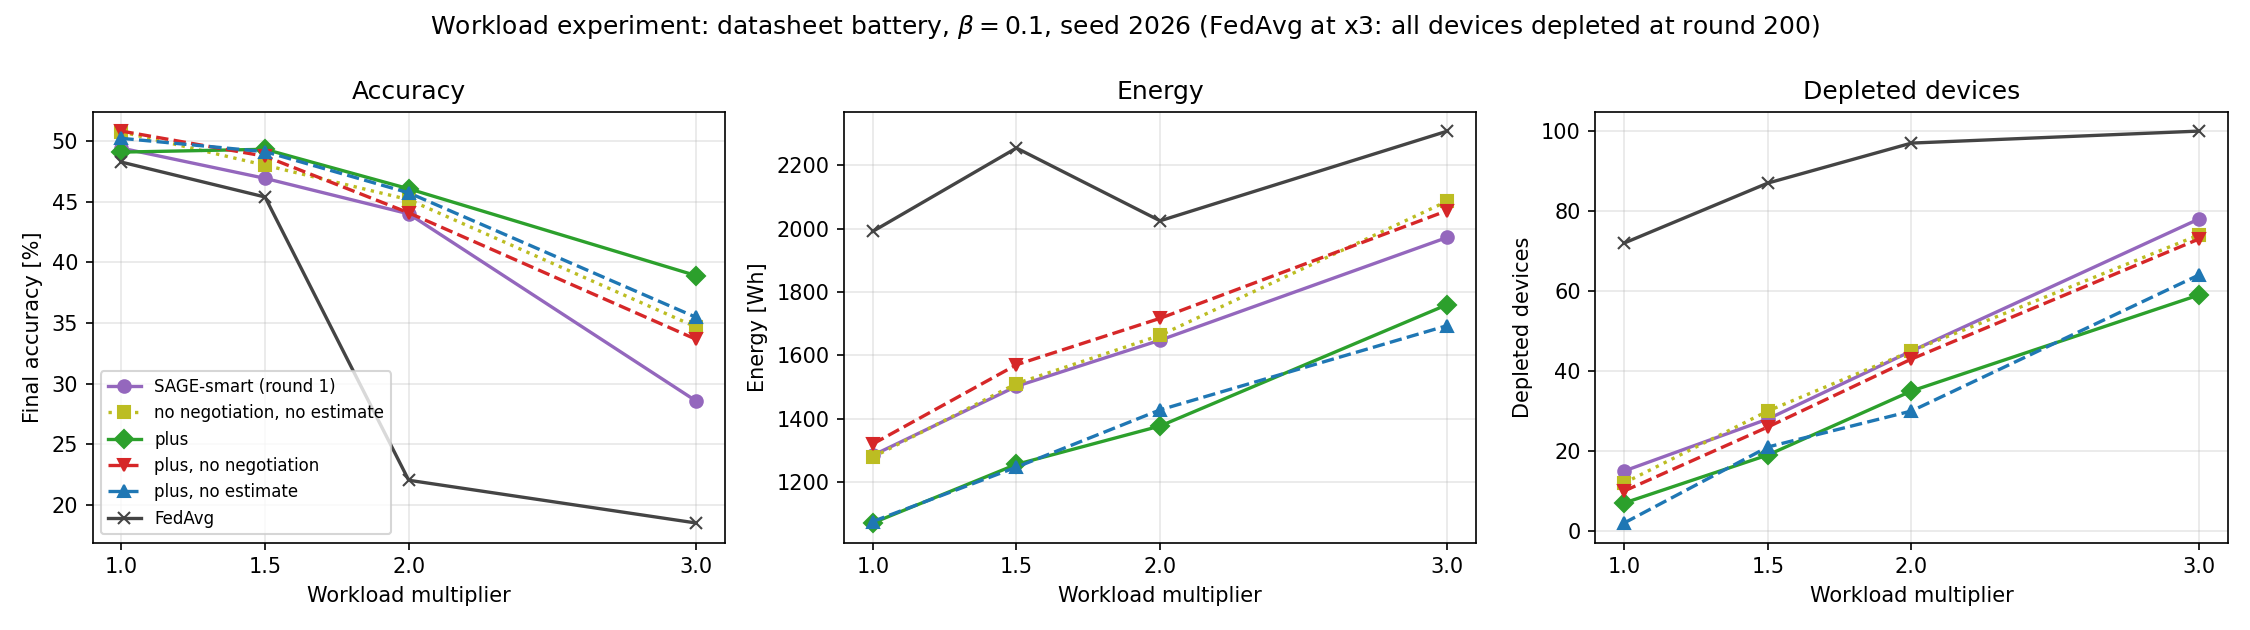
\includegraphics[width=\textwidth]{report14_figs/fig_workload.png}
\caption{Workload experiment: final accuracy, energy and depleted devices against
the multiplier.}
\label{fig:workload}
\end{figure}

\paragraph{Reading.}
\begin{itemize}
  \item \textbf{The diagnosis was right.} Busy clients now refuse before the
        model is sent: late clients fall by a factor of 3--10, rounds are
        26--37\,\% shorter, and less idle energy is spent while waiting.
  \item \textbf{Plus is better than round 1 at every load}: at $\times1$ equal
        accuracy with 17\,\% less energy and half the depleted devices; at
        $\times3$ +10.3 points, 11\,\% less energy and 19 fewer depleted devices,
        and above every variant of round 1.
  \item \textbf{The negotiation now counts}: 14--20\,\% less energy at every
        load, and from $\times2$ also accuracy (+5.2 points and 14 fewer depleted
        devices at $\times3$). In round 1 it was within $\pm$1 point and $\pm$5\,\%.
  \item \textbf{The SoC estimate counts only at $\times3$} (+3.4 points, 5 fewer
        depleted devices, 4\,\% more energy); below, the differences are within
        the noise of one seed.
\end{itemize}

\paragraph{Caveats.}
\begin{itemize}
  \item \textbf{Slow phones with large datasets are excluded.} At $\times1$,
        26\,\% of the proposals are refused, and 8 low-tier phones are never
        selected in the whole run (round 1: none). Five of them are on the low workload
        chain and five start above 80\,\% SoC. With $\beta=0.1$ the local
        datasets differ a lot in size, and a low-tier phone at rest misses the
        deadline only if its dataset is large: 2 epochs never fit, so it refuses
        every time (dataset sizes are not logged). The low tier participates 31 times on average instead
        of 55, and the Gini index of participation goes from 0.32 to 0.43. With
        one seed the accuracy does not suffer, but the data of these phones never
        reaches the model.
  \item \textbf{Most of the gain in depletions comes from the shorter runs.}
        Subtracting the devices that the world without FL loses in the same time,
        the depletions due to FL are 7 $\to$ 6 at $\times1$, 9 $\to$ 8 at
        $\times1.5$, 8 $\to$ 11 at $\times2$ and 13 $\to$ 4 at $\times3$. At
        $\times1$, 165 of the 213~Wh saved are idle. The gain is real (the run
        ends earlier), but it should be presented this way.
  \item \textbf{One seed, one $\beta$.}
\end{itemize}

\paragraph{Proposed fix (to be tested).} The client refuses for the deadline
\textbf{only if the delay is caused by its current load}: it refuses when the
minimum work does not fit in the deadline now but would fit at rest. A client
that does not fit even at rest accepts as in v2. This targets exactly the case
of interest (``I am busy, ask me later'') without excluding anybody for good.
Plan: 2 runs ($\times1$ and $\times3$); if it keeps the gains and nobody is
excluded, it becomes the method, and the 27 SAGE-smart runs of the main
campaign are redone with it.

%======================================================================
\section{Limits}

\begin{itemize}
  \item \textbf{Per-device and time analyses on seed 2026 only}: the runs of
        seeds 42 and 73 copied from the previous campaign have no per-device
        logs and no time column (66 runs, about 3.5 days to redo).
  \item \textbf{FedAvg at $B=16$} still has one seed. At 250 rounds it was
        58.0\,\% with 67 depleted devices against 52.5\,\% and 8 for SAGE-smart,
        but it reached the final accuracy of SAGE-smart already at round 83--100
        with 19--31\,\% less energy (19/10 report). Our advantage over it is the
        batteries, not the energy at equal accuracy.
  \item \textbf{Workload experiment}: one seed, one $\beta$; SAGE-smart plus
        is preliminary and excludes some slow phones (Section~\ref{sec:plus}).
  \item ``Due to FL'' is a difference of counts between two simulations, not a
        per-device attribution.
  \item Depletion is permanent; SAGE-smart is still rising at round 250.
\end{itemize}

%======================================================================
\section{Next steps}

\begin{enumerate}
  \item \textbf{Test the fix of SAGE-smart plus} (refusal for the deadline only
        when due to the current load): $\times1$ and $\times3$, then two more
        seeds at $\times2$ and $\times3$. If confirmed, redo SAGE-smart in the
        main campaign (27 runs, about 1.5 days) and update the method in the
        paper.
  \item \textbf{FedAvg at $B=16$}, seeds 42 and 73, and seed 2026 again with the
        new logs (9 runs); possibly SAGE at $B=16$ as well.
  \item \textbf{Protocol as a run option} (P1 / P2 / P3), combined with the
        workload multiplier ($3\times3$ runs).
  \item \textbf{Paper}: results section, with the equal-accuracy energy and the
        depletion analysis (SAGE-smart's depletions against the background).
  \item Optional: per-device logs for seeds 42 and 73 (66 runs).
\end{enumerate}

%======================================================================
\section*{References}

\begin{itemize}
  \item F.~Maciel et al., ``Federated learning energy saving through client
        selection'' (ESCS), Pervasive and Mobile Computing 103 (2024) 101948.
  \item M.~Savoia et al., ``SAGE: Sustainable and green energy-aware client
        selection for federated learning'', Applied Energy 410 (2026) 127568.
  \item Phones, 4G, recharge and battery: see the 12/10 and 19/10 reports.
\end{itemize}

\end{document}
